\documentclass[10pt,letterpaper]{article}

\usepackage[margin=0.7in]{geometry}
\usepackage{graphicx}
\usepackage{amsmath,amssymb}
\usepackage{enumitem}
\usepackage{titlesec}
\usepackage{hyperref}
\usepackage{booktabs}

\setlength{\parindent}{0pt}
\setlength{\parskip}{4pt}
\setlist{nosep,leftmargin=*}
\titlespacing*{\section}{0pt}{8pt}{4pt}
\titlespacing*{\subsection}{0pt}{6pt}{3pt}
\graphicspath{{phase1_report_figures/}{docs/phase1_report_figures/}}
% Figures copied from results/phase1_v2_batch/ (generated from the raw core runs).

\begin{document}
\begin{center}
    {\Large \textbf{CSE291A: Phase 1 Report}}\\[-1pt]
    {\small Memory-Aware Agent Edge Serving: FIFO Baseline}
\end{center}
\vspace{-8pt}

\section{Question and workload}
Agent tasks issue dependent model requests, pause for tools, and carry growing
conversation histories. On a constrained server, retaining a task's KV cache
may save recomputation but occupy a slot while no model call is ready. We ask
how fixed-concurrency FIFO policies trade completed work, latency, and memory.

We built 80 versioned development tasks and replay a fixed 60-task subset:
\textbf{10 short QA} (SQuAD-derived passages, one model call),
\textbf{10 long-context QA} (deterministic fictional registers with distractors,
one call; 1,803--3,425-token prompts),
\textbf{10 long generation} (five explanations and five stories, one call with
512- or 1,024-token caps), and \textbf{30 multistep} sales, log, document, and
inventory workflows. The multistep tasks have 2, 4, or 7 scripted local tool
calls, hence 3, 5, or 8 dependent model calls. The 60-task replay schedules
182 model calls and 122 tool calls. A tool reveals a fixed fixture after a
configurable delay (2 seconds by default); the model does not choose the tool.
The fictional documents and tool fixtures use fixed seeds; writing prompts
were authored. Offline validators check IDs, answer spans, and fixture
calculations. The runner retains the conversation and records every response.
Exact QA and typed final-JSON references are separated from model inputs;
writing judgments remain partly manual.

\section{FIFO baseline and measurement}
\textbf{Request FIFO} queues each model call and releases its concurrency
permit during a tool wait; a returning agent joins the tail and may need its
history recomputed. \textbf{Task FIFO} admits whole tasks in arrival order,
pins each to a server slot, and retains that slot and its KV cache through
tool waits. We set scheduler concurrency $K\in\{1,2,4\}$ while keeping the
server at four slots and 16,384 total context tokens (4,096 per slot).
Every comparison uses Qwen2.5-7B-Instruct Q4\_K\_M on an AWS g6.xlarge/L4,
batch arrivals, temperature zero, no host RAM cache, and three repeats.
Each run restarts llama-server and performs the same one-request warm-up.
Workload, model, runtime, and source checksums are recorded.

We log task arrival, admission, completion, and tool time; each model request
has queue time, time to first token, generated tokens, and cached/computed
prompt tokens. Task latency is arrival-to-finish; queue time includes admission
and request waits. Throughput is completed tasks divided by replay makespan.
We report p50/p95, failures against all offered tasks, and peak sampled GPU
memory and server RSS (100-ms samples). Outputs and reference scores are kept
with the raw traces. Queue time includes capacity waits, not isolated scheduler
CPU overhead.

\section{Controlled results and interpretation}
Table~\ref{tab:core} and Fig.~\ref{fig:core} summarize the controlled matrix.
\begin{table}[h]
\centering
\small
\setlength{\tabcolsep}{4pt}
\begin{tabular}{@{}lrrrrrrr@{}}
\toprule
FIFO & $K$ & tasks/s & task p50 & task p95 & queue p95 & GPU MiB & correct \\
\midrule
Request & 1 & 0.135 & 187 & 439 & 406 & 5,921 & 33/50 \\
Task    & 1 & 0.091 & 130 & 589 & 570 & 5,917 & 31/50 \\
Request & 2 & 0.155 & 145 & 384 & 331 & 5,923 & 33/50 \\
Task    & 2 & 0.166 &  79 & 321 & 301 & 5,917 & 32/50 \\
Request & 4 & 0.324 &  73 & 184 & 133 & 5,925 & 31/50 \\
Task    & 4 & 0.255 &  54 & 210 & 185 & 5,917 & 31/50 \\
\bottomrule
\end{tabular}
\caption{Median of three repeats per setting; latency and queue columns are
seconds. Each run offered and completed 60 tasks. Correct counts use the 50
automatically judged QA and multistep tasks; 10 writing tasks are unjudged.}
\label{tab:core}
\end{table}

\begin{figure}[h]
\centering
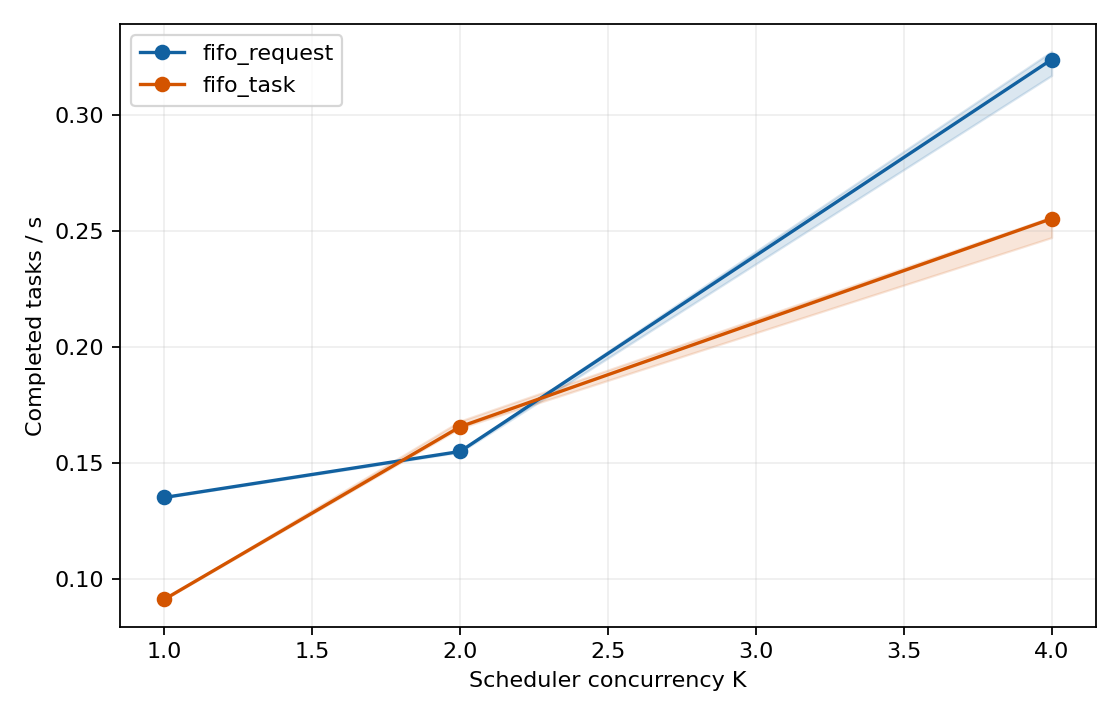
\includegraphics[width=0.49\linewidth]{throughput_completed_tasks_s.png}\hfill
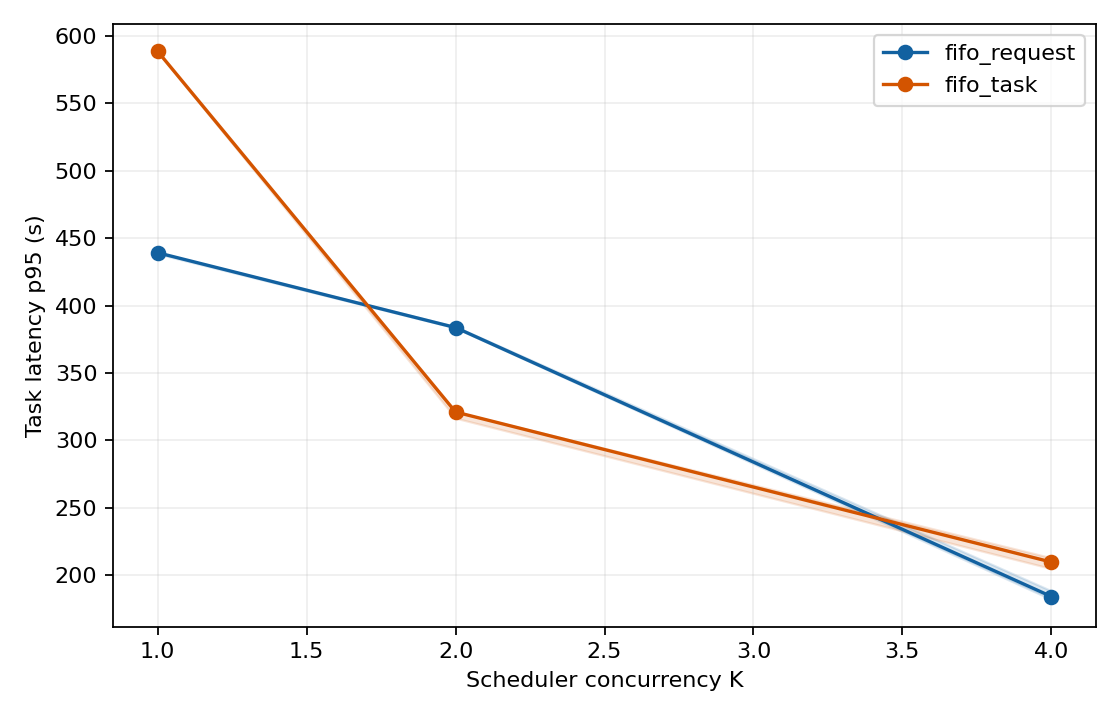
\includegraphics[width=0.49\linewidth]{latency_p95_s.png}
\caption{Completed-task throughput and task p95 versus scheduler concurrency.
Shading spans the three repeats. Server slot count and KV allocation stay fixed.}
\label{fig:core}
\end{figure}

All 18 runs completed all 60 tasks: 1,080/1,080 executions, no model-request
failures or context truncations. Raising $K$ increased throughput for both
policies. At $K=4$, request FIFO completed about 27\% more tasks/s than task
FIFO, while task FIFO had lower median latency (54 versus 73 s) but worse p95
(210 versus 184 s). At $K=2$, task FIFO led throughput by about 7\% and had
lower median and p95 latency. Multistep tasks had much larger queue tails than
short QA in this batch; task order and policy both require examination before
attributing this disparity to starvation.

GPU peaks stayed near 5,920 MiB because the server's KV allocation was fixed.
The measured bottleneck here is substantial waiting and the choice to hold or
release slots, \emph{not observed memory exhaustion}. Median prefix-cache-hit
ratios were 8--10\% for request FIFO and about 66--67\% for task FIFO; this
reflects the different slot-retention policies, not an isolated prefix-sharing
experiment. Automatic correctness was only 31--33 of 50 judged tasks per run;
10 writing tasks per run await semantic judgment, and 66--82 intermediate
agent calls per run hit their output cap. Completion alone therefore does not
establish equal task quality.

\section{Exploratory evidence and next step}
Earlier v1 sweeps suggest where memory management may matter: at a nominal
12k-token synthetic agent document, request FIFO took 352 s versus 146 s for
task FIFO and 144 s for request FIFO with a CPU RAM cache. With 10-second
tool waits on the v1 task mix, task FIFO took 691 s versus 276 s for request
FIFO. A 30k-token microbenchmark measured roughly 1.24 s to restore KV from
RAM versus 14.8 s to recompute it. These are \emph{exploratory}: most v1 cells
ran once, and changing synthetic document size also changed other prompt text.
They motivate, but do not validate, a memory-aware policy.

Controlled context-length, tool-delay, arrival-rate, response-length, and
RAM-cache sweeps are in progress. They will test when recomputation, idle
slots, or host memory dominate. A candidate Phase 2 mechanism is admission
based on estimated KV demand, with priority for ready agent steps; any
cache-aware decision must use controls and counters exposed by llama.cpp.
We will choose one focused policy after these measurements and compare it
against both FIFOs and a tuned fixed-$K$ baseline, including quality and
long-task fairness.

\clearpage
\appendix
\section{Timeline and milestones}
\begin{tabular}{@{}p{0.16\linewidth}p{0.58\linewidth}p{0.17\linewidth}@{}}
\toprule
When & Milestone and evidence & Status \\
\midrule
Nov.\ 3 & Versioned 80-task collection, FIFO runner, reference checks,
AWS smoke and exploratory v1 sweeps. & Complete \\
Nov.\ 4 & Revised v2 prompts; 60-task Qwen validation; fresh-server
protocol and 18-run controlled $K$ matrix with raw traces and curves. & Complete \\
Nov.\ 4--5 & Paired delay, arrival, context, output-length, and RAM-cache
sweeps (56 planned runs); audit failures, memory, output lengths, and quality. & In progress \\
Next & Identify the measured pressure point; implement one memory-aware
policy and compare with both FIFOs and a tuned fixed-concurrency baseline. & Planned \\
\bottomrule
\end{tabular}

\vspace{6pt}
\textbf{Reproduction artifacts.} Task definitions:
\path{workloads/tasks/v2/}; run protocol:
\path{docs/phase1_protocol.md}; raw core traces:
\path{results/raw/phase1_v2_batch_*}; aggregated core metrics and figures:
\path{results/phase1_v2_batch/}. The v1 caveats are documented in
\path{docs/v1_sweep_audit.md}. Exact model and runtime hashes are in each
\path{deployment.json}.

\end{document}
